\documentclass[tikz,border=10pt]{standalone}
\usepackage[utf8]{inputenc}
\usepackage{amsmath, amssymb}
\usetikzlibrary{arrows.meta, positioning, calc, quotes, angles}

\begin{document}

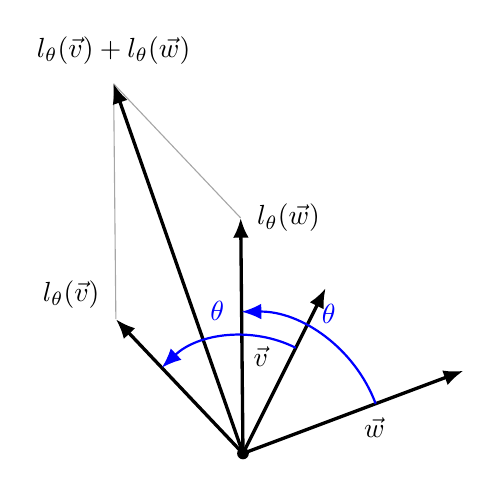
\begin{tikzpicture}[
    thick,
    >={Latex[length=2.5mm, width=2mm]}, % User's preferred arrow style
    dot/.style={circle, fill=black, inner sep=1.5pt, outer sep=2pt}, % User's dot style
    vector/.style={->, very thick}, % Style for main vectors
    helper/.style={gray!70, thin}, % Style for parallelogram lines
    angle arc/.style={->, blue, thick} % Style for the rotation angle
]

    % === Coordinates (using the same v and w as before) ===
    \coordinate (O) at (0,0);
    \coordinate (w) at (2.8, 1.05);   
    \coordinate (v) at (1.05, 2.1);   

    % === Calculate Rotated Vectors (Rotation by 70 degrees) ===
    % Using the same rotation angle as in the previous picture for consistency
    \coordinate (rotated_v) at ($(O)!1!70:(v)$); 
    \coordinate (rotated_w) at ($(O)!1!70:(w)$);

    % === Calculate the Sum of Rotated Vectors ===
    \coordinate (sum_rotated) at ($(rotated_v)+(rotated_w)$); 

    % === Draw Parallelogram Construction for the Sum of Rotated Vectors ===
    \draw[helper] (rotated_v) -- (sum_rotated);
    \draw[helper] (rotated_w) -- (sum_rotated);

    % === Draw Vectors ===
    % Original Vector w
    \draw[vector] (O) -- (w) node[midway, below right, yshift=2pt] {$\vec{w}$};
    
    % Original Vector v
    \draw[vector] (O) -- (v) node[midway, left=2pt, yshift=5pt] {$\vec{v}$};

    % Rotated Vector w
    \draw[vector] (O) -- (rotated_w) node[right, xshift=2pt] {$l_\theta(\vec{w})$};
    
    % Rotated Vector v
    \draw[vector] (O) -- (rotated_v) node[above left, xshift=-2pt] {$l_\theta(\vec{v})$};
    
    % Sum of Rotated Vectors
    \draw[vector] (O) -- (sum_rotated) node[above, yshift=3pt] {$l_\theta(\vec{v}) + l_\theta(\vec{w})$};

    % === Draw Origin Dot ===
    \node[dot] at (O) {};

    % === Draw Rotation Arcs ===
    
    % Arc for v -> rotated_v
    \pgfmathanglebetweenpoints{\pgfpointanchor{O}{center}}{\pgfpointanchor{v}{center}}
    \let\StartAngleV\pgfmathresult
    \pgfmathanglebetweenpoints{\pgfpointanchor{O}{center}}{\pgfpointanchor{rotated_v}{center}}
    \let\EndAngleV\pgfmathresult
    
    \draw[angle arc] (\StartAngleV:1.5cm) arc (\StartAngleV:\EndAngleV:1.5cm) 
        node[midway, above, yshift=2pt, xshift=-3pt] {$\theta$};

    % Arc for w -> rotated_w
    \pgfmathanglebetweenpoints{\pgfpointanchor{O}{center}}{\pgfpointanchor{w}{center}}
    \let\StartAngleW\pgfmathresult
    \pgfmathanglebetweenpoints{\pgfpointanchor{O}{center}}{\pgfpointanchor{rotated_w}{center}}
    \let\EndAngleW\pgfmathresult
    
    \draw[angle arc] (\StartAngleW:1.8cm) arc (\StartAngleW:\EndAngleW:1.8cm) 
        node[midway, above, yshift=1pt, xshift=2pt] {$\theta$};

\end{tikzpicture}
\end{document}
